%%%% PROCESAR con PdfLaTeX !!!!!


\documentclass[12pt]{book}
\usepackage{geometry}\geometry{top=2cm,bottom=2cm,left=3cm,right=3cm}
\usepackage{amssymb}
\usepackage{amsmath}
\usepackage{graphicx}
\usepackage{txfonts}




\begin{document}
\thispagestyle{empty}

\begin {center}

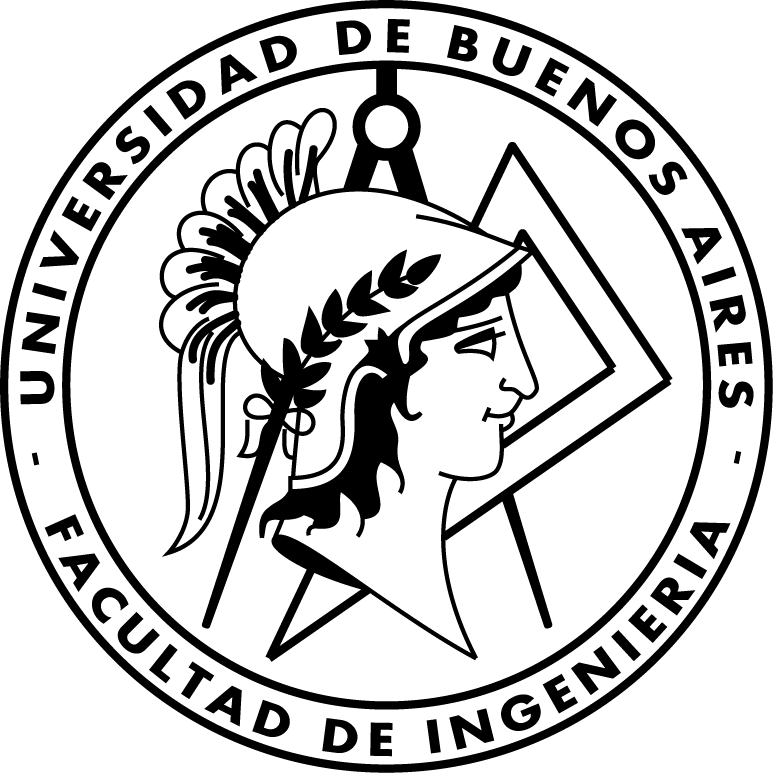
\includegraphics[scale=.4]{Logo-fiuba_big.png}

\medskip
UNIVERSIDAD DE BUENOS AIRES

Facultad de Ingenier\'ia

Departamento de Computaci\'on


\vspace{3cm}


\textbf{\large 7510 T\'ecnicas de Diseño}

\vspace{2cm}


Este trabajo es una recopilacion de resumenes de clase y apuntes de distintas materias de diseño tanto de la UBA como de otras universidades como UTN, para los alumnos de la f\'acultad de ingenier\'ia  de la UBA de las carreras de licenciatura en an\'alsis de sistemas e ingenier\'ia inform\'atica y para todo aquel que se sienta interesado por el diseño de software.
De ninguna man\'era pretende ser una gu\'ia de estudio, ni remplaza las clases presenciales, el material oficial de la catedra esta disponible en el web site de la m\'ateria.
\\
http://materias.fi.uba.ar/7510/

\end {center}


\vspace{2.5cm}

\noindent Autor:\,	Isaac Edgar Camacho Ocampo
 
\noindent Carrera:\,	Licenciatura en An\'alisis de sistemas

\vspace{1cm}

\vspace{1cm}

\noindent Buenos Aires, 2019

\newpage


\tableofcontents

\chapter{Introducción al Diseño}
\section{¿Qué es diseñar?}
\textbf{diseñar es tomar decisiones sobre los componentes de un sistema}, en particular

\begin{itemize}
\item encontrar cuáles son esos componentes 
\item qué responsabilidad tiene cada componente (qué va a hacer, qué no puede resolver, qué va a necesitar que otro le resuelva)
\item cómo se relaciona cada componente con los demás para formar un sistema
\item repasamos la definición de un sistema como "conjunto de partes que se relacionan para lograr un objetivo común".
\end{itemize}
En el paradigma de objetos, los componentes son objetos, las \textbf{responsabilidades} están definidas por la interfaz del objeto. 
\\
Recordamos interfaz vs. implementación; \textbf{interfaz} es lo que le puedo pedir a un objeto que haga (mensaje), \textbf{la implementación} es cómo lo termina resolviendo (método). 
¿Cómo se relacionan los objetos?, enviándose mensajes. 
\\
Pero para eso se tienen que conocer. ¿Y cómo los conozco? Mediante una referencia temporal (variable local, parámetro) o más permanente (variables de instancia o de clase).

\section{Diseño de sistemas y diseño de software}
¿cómo se relacionan entre sí el diseño de sistemas y el diseño de software? ¿qué abarca cada concepto?
El diseño de software está englobado en el diseño de sistemas, que tiene características más generales. Podemos diseñar: el sistema electoral que determina el ganador de una elección, un sistema de inscripción a la facultad, un sistema que entrega documentos de identidad a los ciudadanos,
sistemas de control: ascensores, puentes, cámaras de vigilancia, dispensers, brazos robóticos, etc.
y el software que puede hacer de soporte tecnológico a casi todos los sistemas que mencionamos anteriormente. 
El diseño de software es particularmente interesante por sus características no tangibles.
\\
\\
Hay algunas ideas erroneas instaladas:
\begin{itemize}
\item "Se puede diseñar la funcionalidad sin conocer la tecnología" 
\item "Si estoy diseñando y tiro una línea de código, dejé de diseñar"
\item "Diseñar implica saber UML / saber Enterprise Architect / hacer cajitas".
\item “Se puede programar sin necesidad de diseñar”
\end{itemize}

Nuestro pensamiento es que cuando no bajamos a detalle, cuando ignoramos cuestiones esenciales de la tecnología (arquitectura, paradigmas y lenguajes a desarrollar, etc.), cuando nos queremos abstraer de la programación y la consideramos una tarea menor, "operativa", donde no se piensa, estamos "generando una deuda".
\\
\\
Porque si diseñar es tomar decisiones, descartar decisiones técnicas produce un diseño pobre. Y decimos que diseñar no es hacer diagramas, hacer diagramas es documentar las decisiones que tomé en otro momento. Si no hice el diagrama no quiere decir que no diseñé, en todo caso quiere decir que no está documentado.
\\
\\
\textbf{Ejemplo en clase:} el profesor le pide a un alumno que construya una escalera de madera. ¿Qué preguntas se hace el profesor?
qué cualidades quiero que esa escalera tenga (que sea estable, que sea durable, que se construya rápidamente, qué altura debe tener, cuántos escalones)
qué materiales debo utilizar (definido por la decisión anterior) y cómo voy a especificarlo
al pensar alternativas aparecen restricciones (constraints): de tiempo, de costo, de material que el cliente está dispuesto a comprar, de factibilidad técnica (el grado de experiencia del alumno o sus habilidades con determinadas herramientas afectan en la decisión del tipo de escalera que voy a construir), etc.

En conclusión, el profesor no puede hacer su trabajo sin tener un profundo conocimiento del arte de la carpintería, de cómo hacer un corte, de las técnicas disponibles. No se puede separar la teoría de la carpintería de la práctica. Y en toda decisión tenemos que entender los objetivos, priorizarlos, ver los pros y las contras. Entender cada una de nuestras decisiones a cuáles de nuestros objetivos se aplican.

Como vemos, tomar decisiones sin tener en cuenta el juego de variables que intervienen tiene un costo: en el caso del diseño hay restricciones que impone el usuario, la arquitectura, el paradigma y el lenguaje de programación en el que vamos a implementar y que no es posible soslayar: si estamos haciendo un sistema de reclamos para la municipalidad ¿cómo diseñamos el reclamo de un ciudadano? ¿cómo es posible hacerlo sin saber si el sistema será web o cliente servidor, orientado a objetos o con programación funcional, en un lenguaje que hace chequeo de tipos estático o en otro que no tiene testing automatizado?











\section{Guías para comunicar un diseño}

\textbf{¿En qué lenguaje hablamos cuando estamos diseñando?} En general vamos a utilizar Código y UML
\begin{enumerate}
\item Código
Es un buen momento para recordar que el código es una forma totalmente válida para evitar ambigüedades cuando describimos nuestra solución. Bajar a detalle las partes más relevantes nos va a permitir darnos cuenta de que 
determinado objeto necesite recibir más información o conocer a ciertos objetos
un objeto deba delegar responsabilidades a otro objeto
aparezcan nuevas abstracciones que no habíamos pensado originalmente
etc.
\item UML (Unified Modeling Language) 
es un lenguaje o herramienta de comunicación para las personas que permite representar un modelo (una idea) del sistema real. Recordemos que un modelo es una abstracción que lo expresamos a través de los distintos diagramas: el modelo no es el sistema, sino lo que me interesa representar del sistema.
\end{enumerate}

\chapter{Modelo de dominio}
Una vez que terminamos la fase de análisis de requerimientos ya sea con casos de uso o historias de usuarios, nos enfrentamos con una tarea compleja y poco clara respecto del siguiente paso en el trabajo ¿como convertir esos requisitos en el sistema funcionando es decir las lineas de código?.

Sabemos que el código surgió de un diseño previo. Pero, ¿Cómo surgió el diseño? Es decir como llego desde el modelo de casos de uso al diagrama de clases por ejemplo?
La respuesta es un modelo de análisis, hay que hacer un modelo de análisis para continuar con el trabajo.


\section{Patr\'ones de análisis (jill Nicola)}

MODELO DE ANÁLISIS 
• Objetivo: entender en detalle el negocio y sus reglas 
• Mecanismo utilizado: Patrones de Análisis 


MODELO DE DISEÑO 
• Objetivo: implementar una solución al problema planteado en el análisis más las restricciones impuestas por los requerimientos no funcionales. 
• Mecanismo utilizado: Patrones de Diseño 


Grady booch dice que tenemos como herramientas tres mecanismos.
    • PARTICIÓN: Una funcionalidad compleja dividirla en varias 
    • ABSTRACCIÓN: 
    • ESTABLECIMIENTO DE JERARQUÍAS
\\
Existen dos aspectos en el desarrollo de un sistema, la aplicación y el negocio, la aplicación es el conjunto de operaciones que los usuarios pueden hacer con el software los requerimientos funcionales y los casos de uso asociados a estos dan el alcance de la aplicación, por otro lado el negocio es un sistema dentro de otro, el negocio tiene un dominio y un mundo a su alrededor.
\\
\\
La aplicación permite realizar operaciones sobre los objetos de un modelo que representa el dominio del problema del cual forma parte este sistema, el modelo de negocio es importante porque los objetos que lo constituyen, a partir de su comportamiento harán que al accionar sobre ellos desde la aplicación se logran resultados válidos, Esto se logra a través de la asignación de las reglas de negocio a dichos objetos los cuales controlan que el negocio evolucione según esas reglas.



\chapter{Criterios de Buen Diseño SOLID}
\section{¿Qué es el criterio?} 
El criterio es nuestra herramienta para establecer diferencias y tomar decisiones, el significado de criterio es juicio o la capacidad de las personas para emitir un juicio respecto a algo o alguien de acuerdo a la información con la que cuenta. La etimología de criterio proviene del griego kriterion que significa \textbf{"norma para conocer la verdad"}.
\begin{center}
\textit{Supongamos que queremos construir una casa, ¿como empezamos? compramos materiales, llamamos a unos amigos y les decimos !!Comencemos haber que sale!!! esto seguramente es no tener criterio.
}\end{center}
\begin{center}
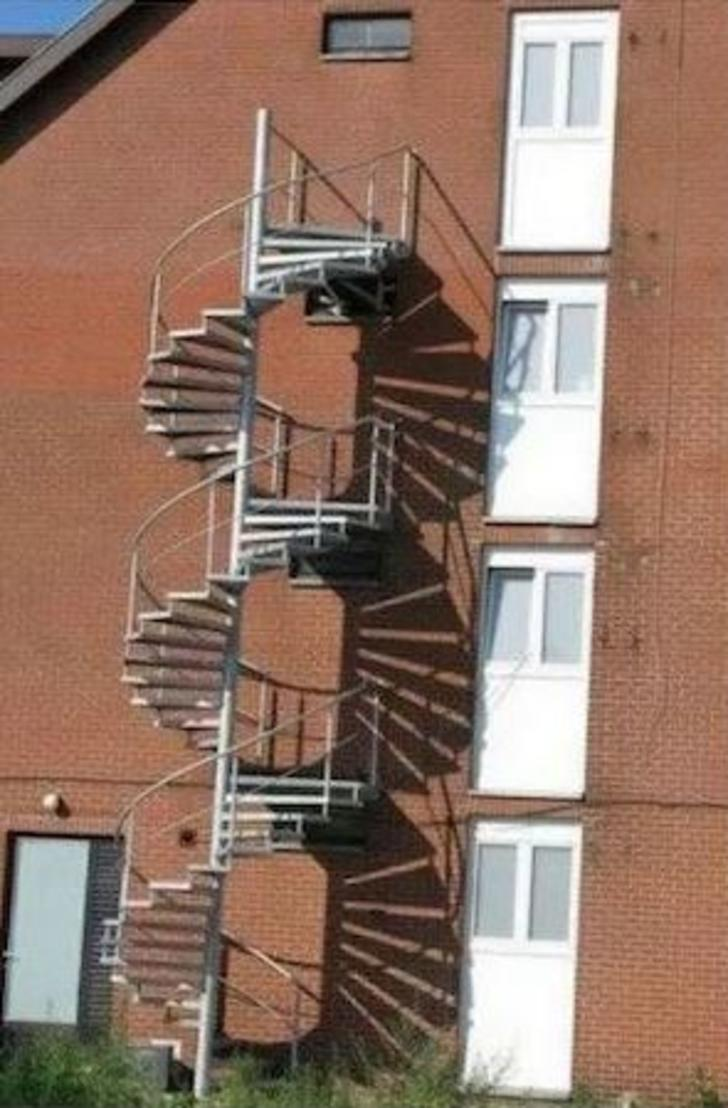
\includegraphics[scale=.3]{job3.jpg}
\end{center}
\section{Diseño}
En el artículo de Robert C. Martín \textbf{The Dependency Inversion Principle} deja en claro lo que es un mal diseño y compara el diseño de software con un trozo de carne que se va descomponiendo conforme pasa el tiempo.
\\
\\
Lo que dice el tio bob es que comparar la ingeniería del Software con la ingeniería civil es una mala comparación porque cada proyecto civil se diseña para no cambiar y la ingeniería del Software trata de modelar una porción de la realidad en la computadora, si queremos que la porción de la realidad modelada sea virtualmente parecida al mundo real, debe necesariamente cambiar, porque la naturaleza del mundo es cambiante, desde ese punto de vista la comparación con el trozo de carne que se va degradando es una buena metáfora.
\subsection{¿Que es un mal diseño?}


Estamos en presencia de un mal diseño cuando esté tiene tres cualidades.
\begin{itemize}
 \item El diseño es rígido.
 \item El diseño es frágil .
 \item Y por último el diseño es inmóvil .
 \end{itemize} Es decir las tres características de un mal diseño es la rigidez la fragilidad y la inmovilidad

\section{Diseño}



\section{Dependencia} En el campo del software una dependencia es una aplicación o una biblioteca requerida por otro programa para poder funcionar correctamente. Por ello se dice que dicho programa depende de tal aplicación o biblioteca.
\\
En UML se dice la clase A depende de la clase B.
\\
\begin{center}
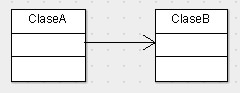
\includegraphics[scale=.5]{dependencia.png}
\end{center}
En el siguiente programa en C++ existe una dependencia con la libreria iostream.\\
\begin{center}
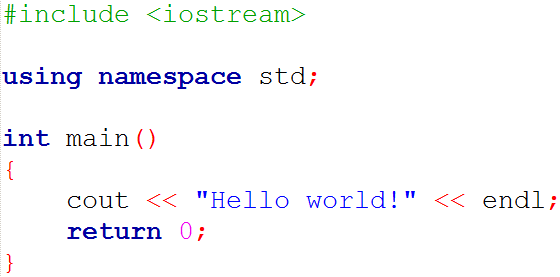
\includegraphics[scale=.5]{Hello_World_C++.png}
\end{center}

\subsection{¿Por qué preocuparse por las dependencias?}
Una dependencia es un riesgo. Por ejemplo, si mi sistema requiere la instalación de un Java Runtime Environment (JRE) y no está instalado, mi sistema no funcionará, Si un progr\'ama en lenguaje C utiliza la libreria "stdio.h" eso tambien es una dependencia y si esa libreria no esta presente ni siquiera va a compilar.
\\
Las dependencias representan riesgo y manejar ese riesgo tiene algún costo que hoy se resuelve a través de la experiencia, prueba y error, o la sabiduría colectiva de un equipo.
\subsection{¿Por que se dice inversion de las dependencias?}
En el análisis y diseño estructurados usabamos la regla de \textbf{divide y vencer\'as}, comenzamos con un problema de alto nivel y lo dividimos en partes más pequeñas. Para cualquiera de esas partes más pequeñas que todavía son "demasiado grandes", continuamos separándolas. El concepto / requisito / problema de alto nivel se divide en partes cada vez más pequeñas. El diseño de alto nivel se describe en términos de estas partes cada vez más pequeñas y, por lo tanto, depende directamente de las partes más pequeñas y más detalladas. Esto también se conoce como diseño de arriba hacia abajo.

\begin{center}
Podemos ver como el m\'odulo principal main se divide en mas funciones \\
de menor nivel y a su vez estas se vuelven a dividir, de esta manera podemos ver que\\
los modulos mas generales dependen de los detalles de implementacion.

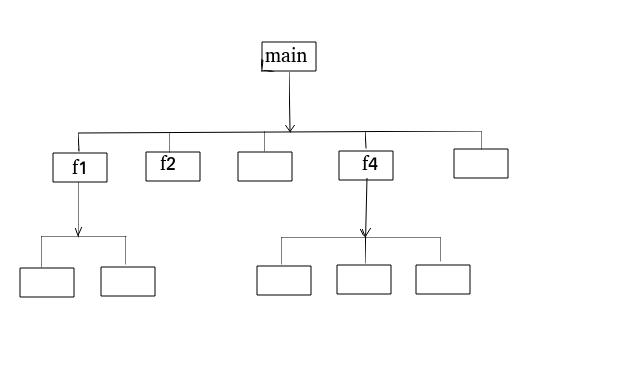
\includegraphics[scale=.7]{dis_estructur.png}
\end{center}

\begin{center}
En el Diseño orientado a objetos tanto los modulos de alto nivel, \\
como los de bajo nivel deben depender de las abstracciones.
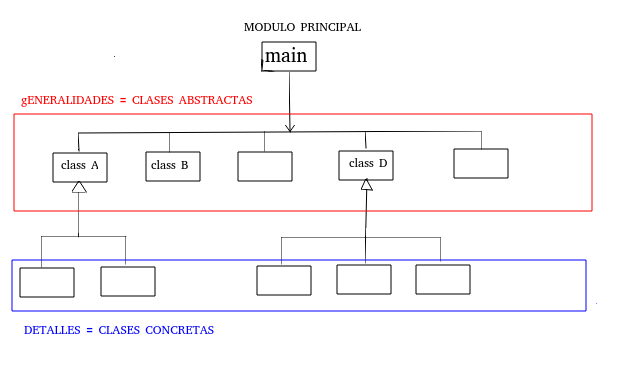
\includegraphics[scale=.7]{dis_OO.png}
\end{center}



\chapter{Parad\'igmas de Programaci\'on}
\section{Paradigma Funcional}


\chapter{Diseño de código}

\chapter{Arquitectura de Software}
\section{Introducción}
\subsection{Patrones de arquitectura}

\chapter{Temas Relacionados}
\section{Docker}
\section{API Rest}
\section{TDD}

\chapter{Patrones de Diseño}
\section{Creacioanles}
\section{De Comportamiento}

\chapter{Métricas}
\textbf{CONCEPTOS PREVIOS}
\begin{enumerate}
	\item \textbf{Eficiencia:} Producir mas con menos recursos o productividad.
	\item \textbf{Eficacia:} Lograr el resultado aunque se consuman muchos recursos.
	\item textbf{Costo de oportunidad:} Es el costo de producir una unidad de un bien.
	\item \textbf{Contribucion marginal:} Ganancia neta.
\end{enumerate}

\chapter{Conclusiones}

\textbf{CONCEPTOS PREVIOS}
\begin{enumerate}
	\item \textbf{Eficiencia:} Producir mas con menos recursos o productividad.
	\item \textbf{Eficacia:} Lograr el resultado aunque se consuman muchos recursos.
	\item textbf{Costo de oportunidad:} Es el costo de producir una unidad de un bien.
	\item \textbf{Contribucion marginal:} Ganancia neta.
\end{enumerate}
\title{\textbf{TRABAJANDO CON MODELOS MATEMATICOS LINEALES}}
\textbf{¿Que es modelizar?} Es hacer una simplificacion de la realidad y nosotros trabajamos con esa simplificacion ya que la realidad es muy compleja.
\\
\textbf{¿Para que hacer un modelo?}
\begin{itemize}
\item \textbf{Economia de recursos:} Al igual que en la ingenieria civil cuando se hacen planos para representar una obra (ya que no seria l\'ogico hacer el edificio y ante un error rehacerlo), cuando modelamos un problema usando programacion lineal y dada la escazes de recursos, es mas eficiente trabajar sobre modelos.
\item \textbf{Eficiencia}: de nuevo so no tengo recursos limitantes entonces trabajo sobre la realidad y no modelo nada.
\item \textbf{simplicidad}: puedo mediante abstracci\'on lograr un modelo mas sencillo y eliminar la complejidad inherente del problema.
\item \textbf{En resumen es mejor que hacer multiples ensayos.}
\end{itemize}
Los mod\'elos se aplican a problemas de desici\'on y este existe cuando existen formas alternativas de actuar, con distintos resultados y diferentes eficiencias para lograr el objetivo es decir existen dudas respecto del curso alternativo a utilizar.
\\
\\
\textbf{Elementos de un modelo}
\\
\\
\textbf{Hipótesis y supuestos:} Para simplificar el modelo se delimita el sistema en estudio a través de las hipótesis y
supuestos simplificativos. Así se comienza a transformar el sistema físico en un modelo simbólico.
Las hipótesis deben ser probadas científicamente. Los supuestos son hipótesis que no pueden probarse.
\\
\textbf{Ejemplos:}
Si estamos modelando una panaderia, y el recurso agua no es limitante y por otro no se dice nada de 				la venta de lo producido podemos agregar las hipotesis
\begin{enumerate}
	\item 	
	\textit{Hay agua suficiente para todos los procesos}
	\item
	\textit{Se vende todo lo que se produce}
\end{enumerate}
\textbf{Objetivo: }Mide la eficiencia de nuestro sistema y lo que buscamos es hallar la merjo solucion. El objetivo surge como respuesta a tres preguntas:
\\¿Qué hacer? es decir que es lo que queremos determinar.
\\¿Cuándo? (período de tiempo) puede ser un mes o año o un periodo t si no se especifica.
\\¿Para qué? para maximizar ganancias, o minimizar costos, nunca ambos a la vez.
\\
\\
\textbf{Actividad}
Proceso unitario que se realiza en el sistema físico caracterizado por consumir recursos
y/o generar un resultado económico y/o indicar un estado, por ejemplo producir un bien o indicar si se finaliz\'o un proceso.
\\
\\
\textbf{Variables}
Son las que miden o indican el estado de una actividad.
Las que miden pueden ser continuas o enteras.
Las que indican son, generalmente, variables (0,1) o bivalentes

\end{document}
